\documentclass{beamer}

\usetheme{Madrid}             % 使用 Madrid 主题
\usepackage{fontspec}
\usepackage{xeCJK}
\usepackage{CJKutf8}
\usepackage{amsmath,amssymb}  % 常用数学环境
\usepackage{hyperref}         % 支持超链接
\usepackage{graphicx}         % 插图
\usepackage{booktabs}         % 表格更好看

\title{NLP与深度学习 - 理论篇}
\subtitle{从n-gram到Attention}
\author{Junchen Feng}
\institute{Generation AI}
\date{\today}

\begin{document}

% 封面页
\begin{frame}
  \titlepage
\end{frame}

% Slide 1
\begin{frame}{课程简介}
  \textbf{课程目标}  
  \begin{itemize}[<+->]
    \item 了解 NLP 从传统 n-gram 到深度学习(word2vec、Attention等)的核心思路
    \item 掌握 Skip-gram 的直观含义、词向量 "\texttt{king - man + woman = queen}" 著名例子
    \item 理解 Seq2Seq、LSTM 与 Attention/Transformer 的基本原理
  \end{itemize}
  \vspace{1em}
  
\end{frame}

% Slide 2
\begin{frame}{示例句子}
  \textbf{示例句子:}
  \begin{block}{}
  \emph{\small
    "I met my friend Sarah yesterday. She told me about her new research project. It might revolutionize the AI field, according to the professor who worked with her last year."
  }
  \end{block}
  \vspace{1em}
  \begin{itemize}[<+->]
    \item \textbf{代词指代}: "She"和"her"指的是 Sarah;"It"指"her new research project"
    \item \textbf{省略/隐含信息}: "the professor" 暗示需要背景,可能在更前面或上下文中
    \item \textbf{长距离依赖}: "her" 多次出现,需要模型能记住之前提到的实体 "Sarah"
  \end{itemize}
\end{frame}

% Slide 3
\begin{frame}{n-gram 模型}
  \textbf{1. 核心思路:}
  \begin{itemize}[<+->]
    \item 通过统计固定大小的词/字符序列出现的频率来表达语言规律
    \item 例如,对句子 "I met my friend Sarah",在 2-gram 中出现 "I met", "met my", "my friend", "friend Sarah" 等
  \end{itemize}
  \vspace{1em}
  \textbf{2. 概率公式(以 n-gram 为例):}
  \[
  P(w_1, w_2, \ldots, w_n) \approx \prod_{i=1}^{n} P(w_i \mid w_{i-1}, \ldots, w_{i-n+1})
  \]
  \vspace{1em}
  \textbf{3. 局限:}
  \begin{itemize}[<+->]
    \item 当句子变得复杂、长度变长(尤其含代词指代),n-gram 往往无法捕捉远距离词的关系,容易出现数据稀疏
    \item 这就是为什么前面那个多重指代的句子里,n-gram 很难"知道" She 和 Sarah 是同一个人
  \end{itemize}
\end{frame}

% Slide 4
\begin{frame}{word2vec 与词向量概念}
  \textbf{1. 为什么要用词向量?}
  \begin{itemize}[<+->]
    \item 传统方法中,词是离散 ID,没有"距离"概念;无法度量语义相似度
    \item \textbf{词向量} 将词映射到连续向量空间,语义相似的词更靠近
  \end{itemize}
  \vspace{1em}
  \textbf{2. 著名例子:}
  \begin{block}{}
    "\texttt{king - man + woman = queen}"
  \end{block}
  \begin{itemize}[<+->]
    \item word2vec 能捕捉到单词间的语义关系:性别、身份等
  \end{itemize}
  \vspace{1em}
  \textbf{什么是连续向量空间?}
  \begin{itemize}
    \item \href{https://projector.tensorflow.org/}{点击查看 TensorFlow Embedding Projector 可视化演示}  
  \end{itemize}

\end{frame}

% Slide 5
\begin{frame}{Skip-gram 目标函数}
  \textbf{1. Skip-gram 核心想法:}
  \begin{itemize}
    \item 给定一个目标词 $(w)$,去预测它上下文中的词
    \item 用这个过程来学习"若两个词经常一起出现,则它们的向量应相似"
  \end{itemize}

  \textbf{2. 数学形式 (示意):}
  \[
    \max \sum_{(w, c)} \log P(c \mid w)
  \]
  其中
  \[
    P(c \mid w) = \frac{\exp(\mathbf{v}_c \cdot \mathbf{v}_w)}{\sum_{c'} \exp(\mathbf{v}_{c'} \cdot \mathbf{v}_w)},
  \]
  \[
    \mathbf{v}_w = w\text{的向量}, \quad \mathbf{v}_c = c\text{的向量}
  \]

  \textbf{3. 直观解释:}
  \begin{itemize}
    \item 当 "Sarah" 与 "She" 在文本中常常成对出现,Skip-gram 会调整它们的向量,让 $\mathbf{v}_{\text{Sarah}}$ 和 $\mathbf{v}_{\text{She}}$ 内积更大,提高 $P(\text{She} \mid \text{Sarah})$
    \item 这样,"相互关联高" 的词向量距离会更近
  \end{itemize}
\end{frame}

\begin{frame}{什么是RNN(循环神经网络)?}
  \textbf{1. 基本概念}
  \begin{itemize}
    \item \textbf{动机}:普通的前馈网络无法很好处理序列数据(如文本、语音),因为输入是\textbf{有序}且长度可变的。
    \item \textbf{循环结构}:RNN在每个时间步(t)接收当前输入 \(x_t\) 和上一个时间步的隐状态 \(h_{t-1}\),更新当前隐状态 \(h_t\)。  
    \[
      h_t = f\bigl(W \cdot [\,x_t,\;h_{t-1}\,] + b\bigr)
    \]
    其中 \(f\) 通常是非线性激活函数(如 \(\tanh\)、ReLU等),\([\,\cdot\,]\) 表示向量拼接。
  \end{itemize}
  
  \textbf{2. 优势}
  \begin{itemize}
    \item 能够在序列的\textbf{时间维度}上"记住"或"传递"信息。
    \item 对语言序列、语音信号等有天然的适配性。
  \end{itemize}
  
  \textbf{3. 局限}
  \begin{itemize}
    \item 当序列过长时,RNN中会出现\textbf{梯度消失或梯度爆炸}问题,导致难以记住"远处"的信息。
  \end{itemize}
\end{frame}



\begin{frame}{RNN运行流程示意-1}
  \textbf{1. 以句子序列为例}
  \begin{itemize}
    \item 对句子 "Sarah wants to show her project":
      \begin{enumerate}
        \item \(x_1\) = "Sarah"的词向量 \(\to h_1\)
        \item \(x_2\) = "wants"的词向量 \(\to h_2\)
        \item \(\dots \dots\)
        \item \(x_5\) = "project"的词向量 \(\to h_5\)
      \end{enumerate}
    \item \textbf{每一步} \(t\):
    \[
      h_t = \mathrm{RNNCell}(x_t,\, h_{t-1})
    \]
  \end{itemize}
  
  \textbf{2. 隐状态传递}
  \begin{itemize}
    \item \(h_t\) 不仅和当前输入 \(x_t\) 有关,也跟历史隐状态 \(h_{t-1}\) 强相关。
    \item 这让网络对序列上下文有了"记忆",比如知道"Sarah"在第1个词时出现。
  \end{itemize}
\end{frame}


  \begin{frame}{RNN运行流程示意-2}
  \textbf{3. 输出层}
  \begin{itemize}
    \item 如果是语言模型,用 \(h_t\) 去预测下一个词;
    \item 如果是分类任务(如情感分析),也可能只用最后一个 \(h_T\)。
  \end{itemize}
  
  \textbf{简单示意图}:
  \[
    x_1 \;\to\;[\mathrm{RNNCell}]\;\to\;h_1 
    \;\to\;\;\ldots\;\to\;h_{T-1} 
    \;\to\;[\mathrm{RNNCell}]\;\to\;h_T
  \]
\end{frame}

% Slide 6
\begin{frame}{LSTM}
  \textbf{1. 为什么需要 LSTM?}
  \begin{itemize}
    \item RNN 在长序列中梯度容易消失,难以记住开头关键信息(如 "Sarah")
    \item LSTM 通过"门"机制,能在更长距离保留上下文
  \end{itemize}

  \textbf{2. 核心公式(简示):}
  \[
    f_t = \sigma(\dots), \quad
    i_t = \sigma(\dots), \quad
    C_t = f_t C_{t-1} + i_t \tilde{C}_t, \dots
  \]
  \begin{itemize}
    \item 避免过多细节,聚焦概念掌握
  \end{itemize}

  \textbf{在我们的例子中...}
  \begin{itemize}
    \item 在 "Sarah …… She" 相距较远的情况下,LSTM 可以将最初 "Sarah" 的信息保存在单元状态 $C_t$ 中较长时间
  \end{itemize}
\end{frame}

% Slide 7
\begin{frame}{Attention 机制 - 核心概念}
  \textbf{1. 为什么需要 Attention?}
  \begin{itemize}
    \item LSTM 在非常长距离依赖上仍会有困难
    \item \textbf{Attention}: 让模型在生成某个词时,显式地"查看"输入序列中最相关的部分
  \end{itemize}
  \vspace{1em}
  \textbf{2. Q、K、V 具体解释:}
  \begin{itemize}
    \item \textbf{Query (Q)}: 解码器(或自注意力)当前正在生成的查询向量
    \item \textbf{Key (K)、Value (V)}: 编码器输出(或序列中每个 token)的键和值向量
    \item Attention 分数 = $\text{softmax}\Bigl(\frac{Q K^T}{\sqrt{d_k}}\Bigr)$
    \item 通过分数加权"值"向量,聚焦最相关内容
  \end{itemize}
  \vspace{1em}
  \textbf{3. 优势:}
  \begin{itemize}
    \item 并行计算,且可针对不同位置进行加权
    \item 捕捉远程依赖更灵活
  \end{itemize}
\end{frame}

% Slide 8
\begin{frame}{Attention 演示 (QKV 计算)}
  \textbf{示例:}
  \begin{block}{}
    句子: "Sarah wants to show her project to the professor"
  \end{block}
  \begin{itemize}
    \item \textbf{Query}: Decoder 正在生成 "her",想找到先行词;Q 可以是 "her" 的隐藏向量
    \item \textbf{Key/Value}: 对应编码器对各词的向量表示:["Sarah", "wants", "to", "show", "her", "project", "to", "the", "professor"]
  \end{itemize}
  \vspace{1em}
  \textbf{演示计算} (简化成 1 维):
  \begin{enumerate}
    \item 假设 $Q, K, V$ 均为 1 维向量:
      \[
        Q("her") = 2.0, \quad K("Sarah")=1.5, \; K("her")=2.0, \dots
      \]
    \item 注意力得分 = $Q \times K$ (再除以 $\sqrt{d_k}$, 此处 $d_k=1$):
      \[
        \text{Score("Sarah")} = 2.0 \times 1.5 = 3.0, \quad
        \text{Score("her")} = 2.0 \times 2.0 = 4.0
      \]
    \item \texttt{softmax} 归一化得到注意力权重
    \item 加权合并 $V$ 向量:$\sum_j \alpha_j \times V_j$
  \end{enumerate}
  \vspace{1em}
  \textbf{解释}:
  \begin{itemize}
    \item 若 "her" 与 "Sarah" 或之前的 "her" 相关性最高,则对应的注意力权重最高
    \item 能更好解析指代关系
  \end{itemize}
\end{frame}

\begin{frame}{BERT:双向Transformer预训练模型-1}

  \textbf{1. BERT是什么?}
  \begin{itemize}
    \item \textbf{全名}:Bidirectional Encoder Representations from Transformers
    \item \textbf{提出者}:Devlin et al., 2018/2019
    \item \textbf{核心思路}:基于 Transformer 的 Encoder 部分进行双向预训练;在海量文本上学习语言理解能力,随后可微调(fine-tuning)到各种下游 NLP 任务。
  \end{itemize}
  \vspace{1em}

  \textbf{2. 训练目标}
  \begin{itemize}
    \item \textbf{Masked Language Modeling (MLM)}:随机 \texttt{mask} 掉部分单词(如 15\%),让模型预测被 \texttt{mask} 的词;模型需学会双向关注上下文。
    \item \textbf{Next Sentence Prediction (NSP)}:判断两句话是否前后相邻,从而学习上下句关系。  
      \begin{itemize}
        \item 许多后续工作(如 RoBERTa)取消了 NSP,但 MLM 仍是核心。
      \end{itemize}
  \end{itemize}
\end{frame}


  \begin{frame}{BERT:双向Transformer预训练模型-2}

  \textbf{3. BERT与长距离依赖}
  \begin{itemize}
    \item BERT 使用多层 Transformer Encoder,自注意力机制允许在任意位置直接关注序列中的其他词。
    \item 因为是双向,能同时从前后文获取信息,对上下文理解更出色。
  \end{itemize}
  \vspace{1em}

  \textbf{(可配图/示意)}:
  \begin{itemize}
    \item \textbf{BERT 结构图}:多层 Encoder 堆叠,每层包含多头自注意力和前馈网络。
    \item \textbf{MLM 例子}:"The [MASK] is good." → 模型预测被遮住的单词 "food"。
  \end{itemize}

\end{frame}
\begin{frame}{BERT 架构示意图}
  \begin{figure}
    \centering
    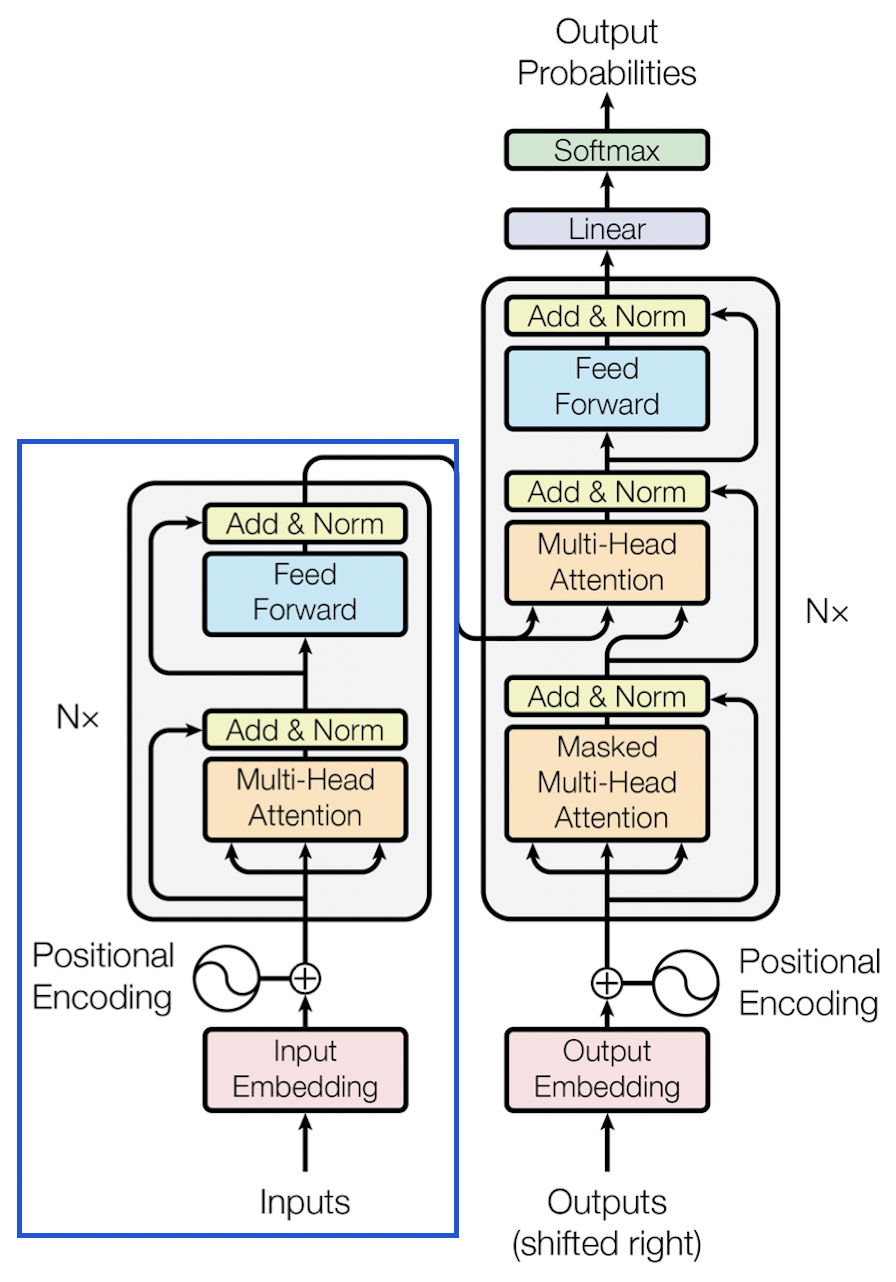
\includegraphics[width=0.6\textwidth, height=0.6\textheight]{BERT4.png}
    \caption{BERT 模型架构图}
  \end{figure}
  
\end{frame}

% Slide 9
\begin{frame}{总结}
  \textbf{1. 回顾}
  \begin{itemize}
    \item \textbf{n-gram}: 简单统计,长距离依赖困难
    \item \textbf{word2vec}: 词向量让 "she" 和 "Sarah" 在语义空间更接近
    \item \textbf{LSTM}: 门机制保留较长依赖信息,但仍有一定局限
    \item \textbf{Attention}: 显式对句子各位置"加权关注",并行化好
    \item \textbf{BERT}: 双向Transformer预训练模型,能捕捉长距离依赖,开箱即用

  \end{itemize}

  \textbf{2. 预告}
  \begin{itemize}
    \item 将用 IMDB 情感分析数据进行实践
    \item 比较传统NLP,简单RNN和BERT的表现
  \end{itemize}
\end{frame}

% Slide 10
\begin{frame}{参考文献 \& 感谢聆听}
  \textbf{1. 关键论文:}
  \begin{itemize}
    \item \textbf{n-gram/语言模型}: Shannon, C. E. (1948). \emph{A mathematical theory of communication.}
    \item \textbf{word2vec}: Mikolov, T. et al. (2013). \emph{Distributed Representations of Words and Phrases and their Compositionality.} NIPS.
    \item \textbf{Attention}: Bahdanau, D. et al. (2014). \emph{Neural Machine Translation by Jointly Learning to Align and Translate.} ICLR.
    \item \textbf{Transformer}: Vaswani, A. et al. (2017). \emph{Attention Is All You Need.} NIPS.
  \end{itemize}
\end{frame}

\begin{frame}{NOTES}
  - 进行贝叶斯概率公式的铺垫
  - 增加RNN的更详细讲解
  - 增加Transformer的讲解

  
\end{frame}


\end{document}
